\documentclass [11pt, a4wide, twoside]{article}

\usepackage{times}
\usepackage{epsfig}
\usepackage{ifthen}
\usepackage{xspace}
\usepackage{fancyhdr}
\usepackage{hyperref}
\usepackage{pdfpages}
\usepackage{amsmath}
\hypersetup{
    % true means draw the links themselves colored and do not draw a bounding
    % box
    colorlinks=true,
    linkcolor= blue,
    citecolor= blue,
    filecolor=blue,
    urlcolor= blue
}

% solution switch
\newboolean{showsolution}
\setboolean{showsolution}{true} %set it either to true or false


%layout
\topmargin      -5.0mm
\oddsidemargin  6.0mm
\evensidemargin -6.0mm
\textheight 215.5mm
\textwidth      160.0mm
\parindent        1.0em
\headsep          10.3mm
\headheight        12pt
\lineskip    1pt
\normallineskip     1pt

%header
\lhead{Programming Languages \\ 2021}

\rhead{Prof. O. Nierstrasz\\
Mohammadreza Hazhirpasand, Joel Niklaus}
\lfoot{page \thepage}
\rfoot{\today}
\cfoot{}

\renewcommand{\headrulewidth}{0.1pt}
\renewcommand{\footrulewidth}{0.1pt}

\renewcommand{\thesubsection}{\arabic{subsection}}

%enumeration
\newenvironment{myitemize}{%
     \begin{itemize}
     \setlength{\itemsep}{0cm}}
     {\end{itemize}}

\newenvironment{myenumerate}{%
     \begin{enumerate} \setlength{\itemsep}{0cm}}
     {\end{enumerate}}


%solution
\ifthenelse{\boolean{showsolution}}
   {  \newcommand{\solution}[1]{
   	\noindent\underline{\textbf{Answer:}}\\[2mm]
   	 \textsl{#1}
	 \vspace{10pt}
	 \normalsize
	}
  }
  {  \newcommand{\solution}[1]{} }

\newcounter{exnum}
\def\xexercise{\fontsize{12}{10}\fontseries{bx}\selectfont}
\def\xnormal{\fontseries{m}\fontshape{n}\selectfont}


\newcommand{\exercise}[1]{%
     {\addtocounter{exnum}{1}\vskip 0.8cm{\xexercise \noindent Exercise
\arabic{exnum} (#1)} \xnormal} \vskip 0.3cm} 
 \newcommand{\aufgabe}[1]{
     {\addtocounter{exnum}{1}\vskip 0.8cm{\xexercise \noindent Aufgabe
\arabic{exnum} (#1)} \xnormal} \vskip 0.3cm} 

\pagestyle{fancy}


% ===============ABBREVIATIONS==============================
\newcommand{\eg}{\emph{e.g.,}\xspace}
\newcommand{\ie}{\emph{i.e.,}\xspace}
\newcommand{\etc}{\emph{etc.}\xspace}


\begin{document}

% title
\section*{\ifthenelse{\boolean{showsolution}}{Solution}{}\space{} Stack-based Programming}

% - - - - - - - - - - - - - - - - - - - - - - - - - - - - - - - - - - - - - - -

\subsection*{Instructions:}

Solutions should be placed in a separate folder with the name ``Assignment02''.\\
Answers to the Exercise 1 submit in \textbf{one} .txt file, clearly marked which answer corresponds to which question.\\
Answers to the Exercises 2 and 3 submit in \textbf{two} .ps files named, accordingly, ``catalan.ps'' and ``stars.ps''.

\subsection*{Exercise 1 (1.5 points)}
Answer the following questions about Postscript:

\begin{myitemize}

\item What kinds of stacks does PostScript manage and what are their roles?

\solution{
\begin{enumerate}
\item Operand stack - the most important, since it's used for all computations
\item Dictionary stack - holds sets of local variables to be used by procedures we define
\item Execution stack - hidden from the user; used to manage running procedures
\item Graphics state stack - makes easy for a user to work in different coordinate systems
\end{enumerate}
}

\item What is the way of defining a procedure in the PostScript program?

\solution{Procedures are defined by binding names to executable objects, in a way ``key value def''.}

\item What are the roles of a dictionary and the dictionary stack in the PostScript program execution?

\solution{By defining our own dictionary, and pushing it to the dictionary stack, we make sure that the names we use do not conflict with any other similar names used by other procedures.
The dictionary stack therefore serves the same purpose as the run-time stack in most programming languages.}
\end{myitemize}

\subsection*{Exercise 2 (2 points)}

Define a procedure in PostScript that will calculate and print the first \texttt{n} \href{https://en.wikipedia.org/wiki/Catalan_number}{Catalan numbers}, where \texttt{n} is an argument on the stack. Catalan numbers are calculated based on the formula $C_{n} = \dfrac{(2n)!}{(n+1)!n!}$.
The call to the procedure should look like \texttt{ n catalan }.
The output should be similar to the one shown in \autoref{fig:catalan} for \texttt{n = 17}.
Please use the provided \href{http://scg.unibe.ch/download/lectures/pl2018-exercises/Assignment02-catalan-template.txt}{template} which contains the skeleton of the code, as it will make it easier for you (and us) to check your solution.
Try to define sub-procedures whenever it makes sense. 

\solution{\href{http://scg.unibe.ch/download/lectures/pl2018-exercises/Assignment2-catalan-solution.ps}{Catalan numbers - solution.}}

\begin{figure*}[h]
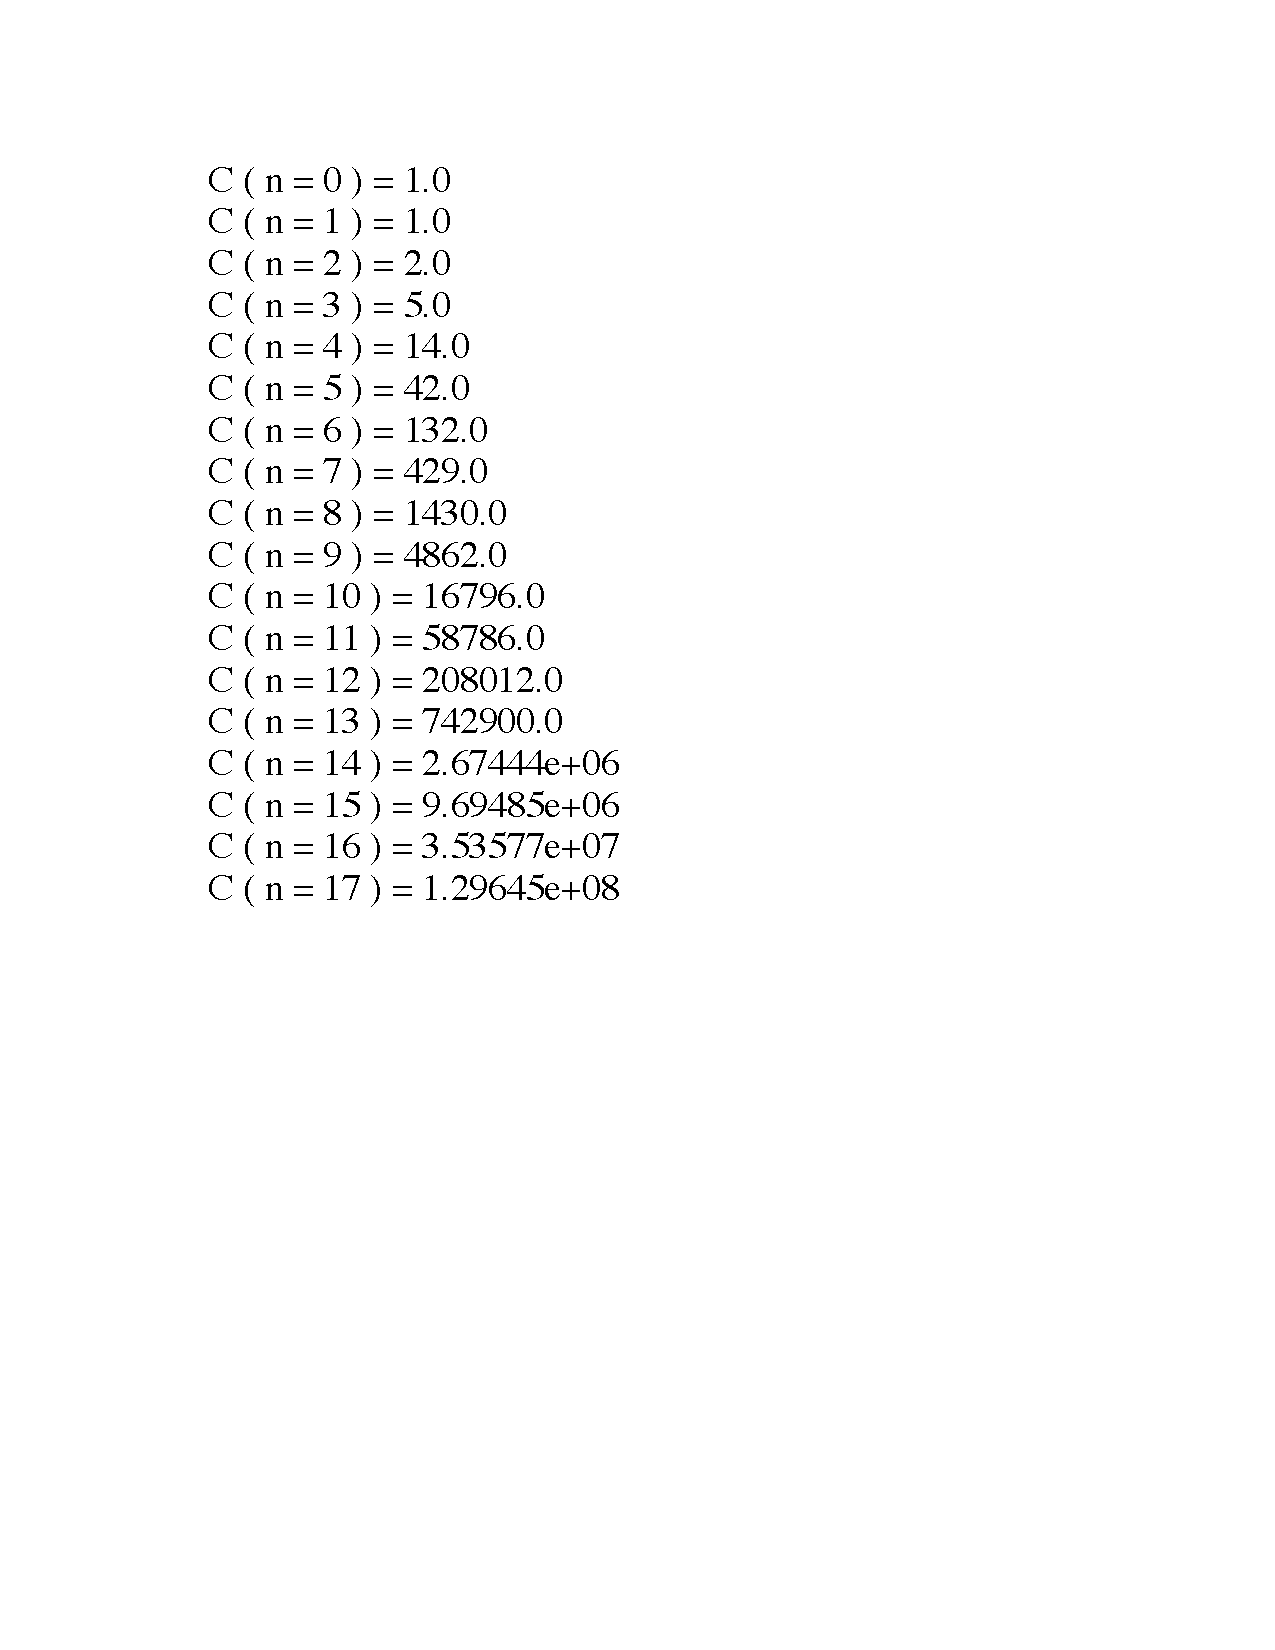
\includegraphics[width=0.358\linewidth]{figs/catalanNumbers.pdf}
\caption{Catalan numbers}
\label{fig:catalan}
\end{figure*}

\subsection*{Exercise 3 (2.5 points)}

Define a procedure in PostScript that will draw five-point stars given the following arguments on the stack:

\begin{description}
\item [\texttt{x}] x coordinate of the center of stars
\item [\texttt{y}] y coordinate of the center of stars
\item [\texttt{radius}] distance from the center of stars to the points of the largest star
\item [\texttt{n}] number of stars
\end{description}

The procedure should draw \texttt{n} stars with the same center, where each star is smaller than the previous one.
The decrease in the distance between the center of a star and the star's points should be by $\dfrac{\texttt{radius}}{\texttt{n}}$.
The largest star should be filled with the black color. 
The each following star should be filled with the brighter nuance of the grey color. The nuance of the grey color of the \mbox{\texttt{i}-th} star should be $\dfrac{\texttt{i}}{\texttt{n}}$. Since we consider the largest star to have the index of \texttt{0}, its nuance of the grey color is $\dfrac{\texttt{0}}{\texttt{n}}$, that is black.


The output should be similar to the one shown in \autoref{fig:stars}, that is the result of the execution 
\begin{verbatim}
300 400 200 10 draw
\end{verbatim}
Please use the provided \href{http://scg.unibe.ch/download/lectures/pl2018-exercises/Assignment02-stars-template.txt}{template} which contains this code, as it will make it easier for you (and us) to check your solution.
Try to define sub-procedures whenever it makes sense. 

\solution{\href{http://scg.unibe.ch/download/lectures/pl2018-exercises/Assignment2-star-solution.ps}{{Star - solution.}}}

\begin{figure*}[h]
\begin{center}

\includegraphics[width=0.5\linewidth]{figs/star.pdf}
\caption{Stars}
\label{fig:stars}
\end{center}
\end{figure*}

\end{document}
